%%%%%%%%%%%%%%%%%%%%%%%%%%%%%%%%%%%%%%%%%%%%%%%%%%%%%%%%%%%%%%%%%%% 
%                                                                 %
%                            CHAPTER                              %
%                                                                 %
%%%%%%%%%%%%%%%%%%%%%%%%%%%%%%%%%%%%%%%%%%%%%%%%%%%%%%%%%%%%%%%%%%% 

\chapter{Background information on DNA and DNA sequencing}
\label{ch:MBbackground}

\section{Biology and DNA}

\subsection{History of genetics and DNA}

\paragraph{Genetics}

\begin{wrapfigure}{R}{0.25\textwidth}
	%src: https://upload.wikimedia.org/wikipedia/commons/8/87/Gregor_Mendel_portrait.jpg
	\begin{center}
		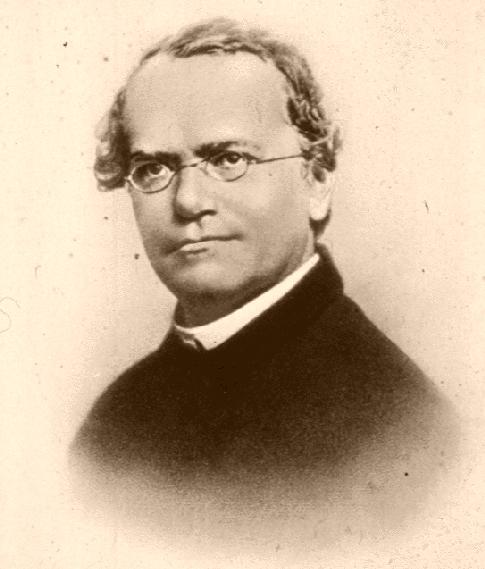
\includegraphics[width=0.20\textwidth]{background/GregorMendel.jpg}
		Gregor Mendel
	\end{center}
\end{wrapfigure}


For thousands of years, humans have observed the effects of heredity and implemented their knowledge to domesticate plants and animals. However, the science behind heredity was only started to be understood since 1859 with the publication of \emph{on the origin of species} by Charles Darwin. 

Around 1865, an Austrian monk and botanist Gregor Mendel, who studied at the university in Brno in the current Czech Republic, published his results on the hybridization studies of pea plants. He is often credited as being the father of modern genetics. In his findings, he implemented the role of \emph{factors} that influence the expression of traits. These factors later became known as \emph{genes}.

\paragraph{DNA}

In 1869, Swiss physician Friedrich Miescher discovered a microscopic substance in the pus of discarded surgical bandages. Later, in 1909, Phoebus Levene named this substance DeoxyriboNucleic Acid (DNA) since it is found in the nucleus of a cell and has acidic properties.

The full structure of DNA was discovered by Francis Crick and James Watson at the Cavendish Laboratory at the University of Cambridge.

\subsection{Structure of DNA}

DNA, or Deoxyribonucleic Acid, is the molecule that stores the genetic information of all living organisms. It is the information that programs all of the activities in a cell.

Structurally, DNA is a polymer, which means each molecule is built up out of small repeating molecular units. In DNA, these units are called \emph{nucleotides}.

\begin{figure}[H]
	\centering
	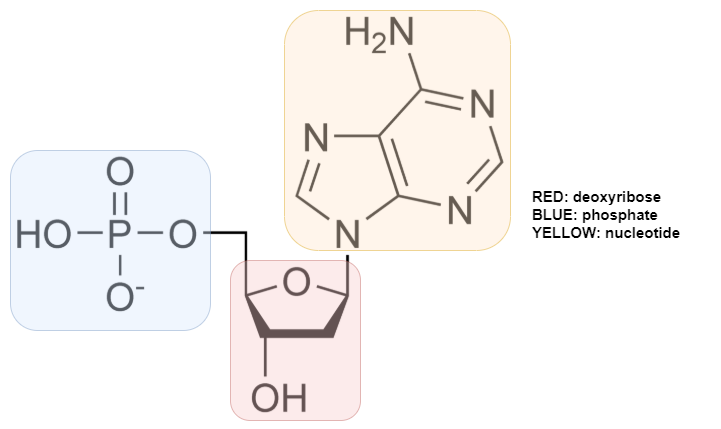
\includegraphics[width=0.75\linewidth]{background/Nucleotide.png}
	\caption{The structure of one nucleotide}
	\label{fig:nucleotide}
\end{figure}

Each nucleotide consists of 3 parts:

\begin{enumerate}
	\item A carbon sugar molecule called \emph{Deoxyribose}.
	\item A phosphate group to connect the Deoxyribose molecules. 
	\item One of four possible nitrogen bases: Adenine ($A$), Thymine ($T$), Cytosine ($C$) or Guanine ($G$).
\end{enumerate}

It is important to note that in most living organisms DNA does not exist as a single polymer, but rather a pair of molecules that are held tightly together. This is the famous \emph{double helix}.

\begin{figure}[H]
	%src: https://upload.wikimedia.org/wikipedia/commons/thumb/1/14/Double_stranded_DNA_with_coloured_bases.png/1024px-Double_stranded_DNA_with_coloured_bases.png
	\centering
	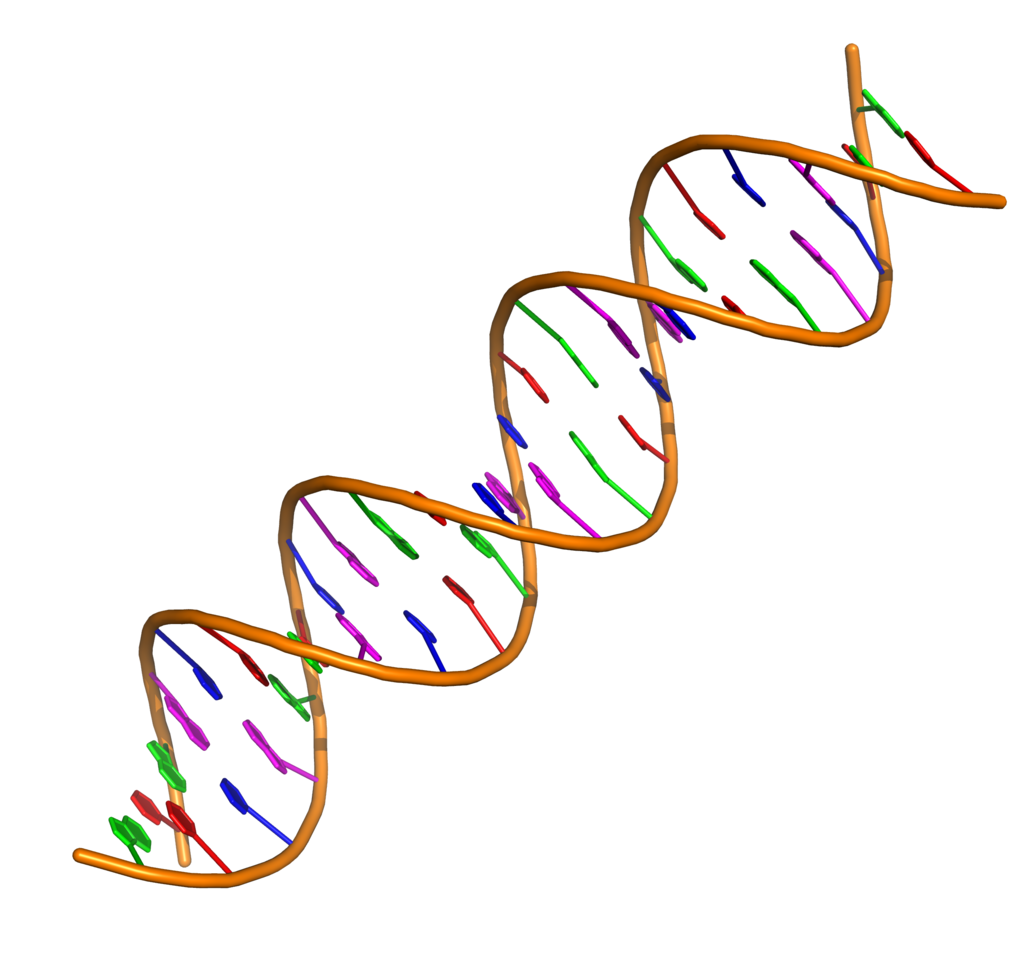
\includegraphics[width=0.3\linewidth]{background/DoubleHelix.png}
	\caption{The famous double helix}
	\label{fig:doubleHelix}
\end{figure}

Like in any good structure, there is a need for the main support. In DNA, the sugars and phosphates bond together to form twin backbones. These sugar-phosphate bonds run down each side of the helix, but chemically in opposite directions. 

The first phosphate group, at the start of the molecule, connects to the sugar group's 5th carbon ($5'$). At the end of the structure, the 3rd carbon ($3'$) of the sugar group is unconnected. This makes a pattern typically noted as $[5' \rightarrow 3']$. Now, since the other molecule in the helix goes in the opposite direction, the pattern of the other backbone is typically noted as $[3' \rightarrow 5']$.

\begin{figure}[H]
	%src: https://upload.wikimedia.org/wikipedia/commons/thumb/e/e4/DNA_chemical_structure.svg/800px-DNA_chemical_structure.svg.png
	\centering
	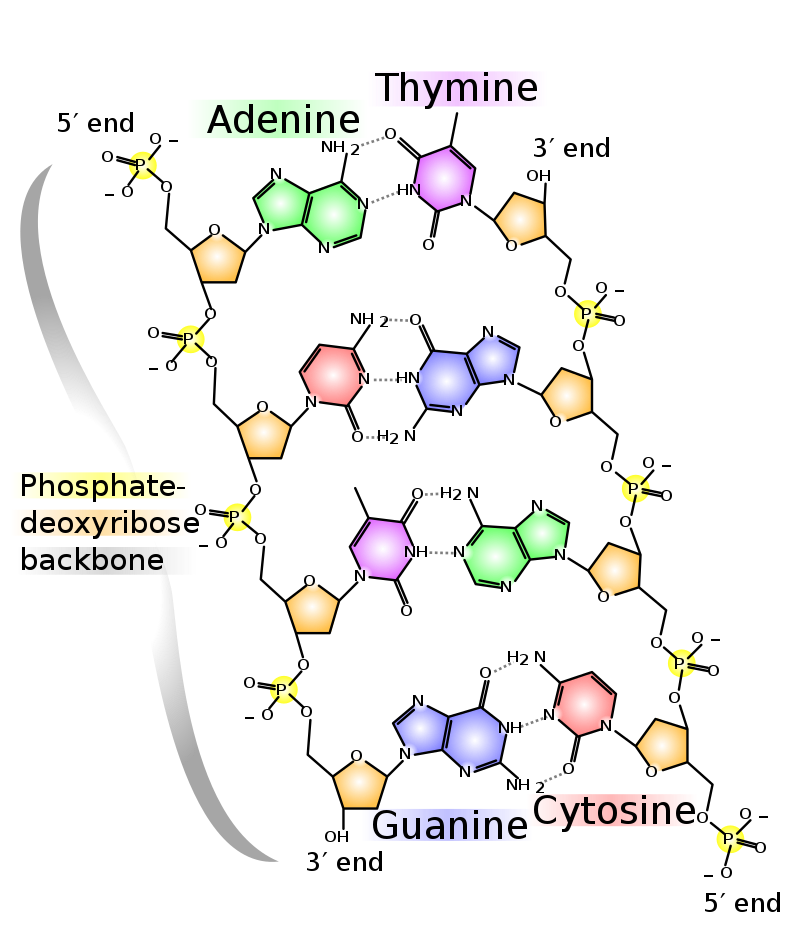
\includegraphics[width=0.5\linewidth]{background/DNAstructure.png}
	\caption{A short part of a DNA molecule containing a $[5' - ACTG - 3']$ (left) and a complementary strand of $[3' - TGAC - 5']$ (right). These 2 strands are interconnected by hydrogen bonds}
	\label{fig:DNAstructure}
\end{figure}

These two long chains are linked together by the nitrogen bases via their relatively weak hydrogen bonds, but there can't just be any pair of nitrogen bases. Adenine can only make hydrogen bonds with Thymine. Likewise, Guanine can only bond with Cytosine. These bonded nitrogen bases are called \emph{base paires}.

It is the order of these bases, which is also called the \emph{sequence}, that allows this DNA to store useful information. In this way, e.g. $AGGTCCATG$ means something completely different as a base sequence than e.g. $TTCCAGATC$.

Since each of the bases in the sequence has only one possible counterpart, you can predict what its matching counterpart will be in the opposite string. For example:

If the following sequence is known
$$[5' - AGGTCCG - 3']$$
we can deduce the sequence in the other direction as
$$[3' - TCCAGGC - 5']$$

\subsection{DNA in the human body}

In human cells, DNA molecules can be found in the nucleus of all cells in the body. It consists of 46 very long molecules, which during cell division condense in what we call \emph{chromosomes}. The only exception is in reproductive cells (the egg cell and the sperm cell), which only have 23 chromosomes. 

The 23 chromosomes, which make up our whole DNA, are always present in pairs in the cells, making a total of 46 chromosomes. Each time, the pair consists of one chromosome from the father and the other one from the mother. 

The 23 chromosome pairs are classified in:
\begin{itemize}
	\item 22 pairs of autosomal chromosomes, marked 1 to 22 according to the length of the sequence. The longest chromosome (chromosome number-1) is 248,956,422 bases long. The shortest (chromosome number-22) is 50,818,468 bases long.
	\item In each cell, there is also an X chromosome plus an X or Y chromosome, dependent on the gender (XY for male, XX for female).
\end{itemize}


\begin{figure}[H]
	%src: https://upload.wikimedia.org/wikipedia/commons/thumb/b/b2/Karyotype.png/800px-Karyotype.png
	\centering
	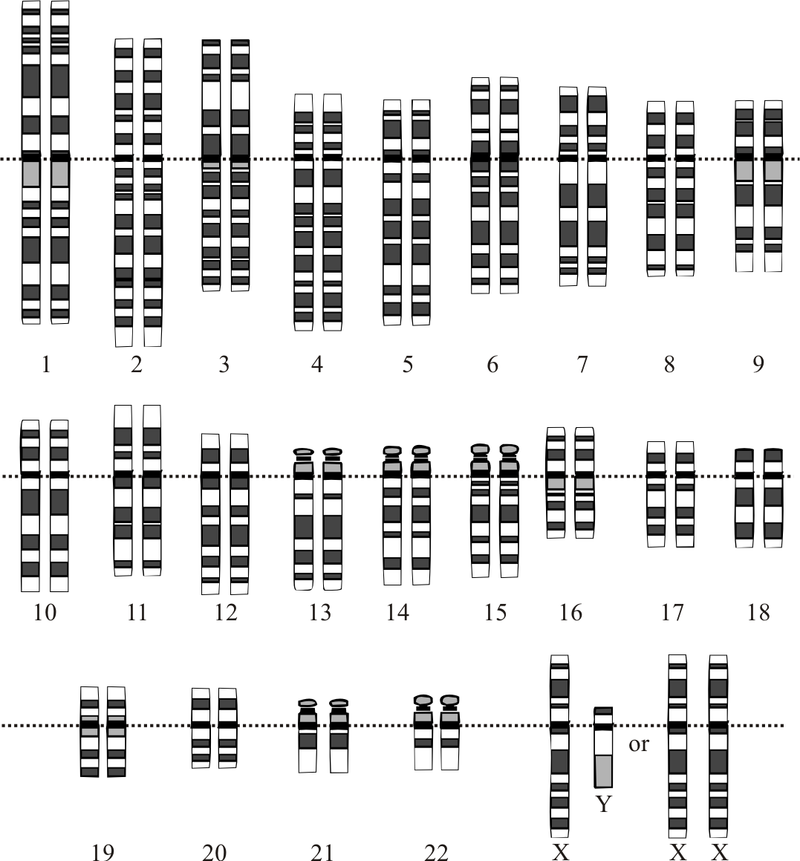
\includegraphics[width=0.5\linewidth]{background/karyotype.png}
	\caption{the 46 human chromosomes}
	\label{fig:karyotype}
\end{figure}

These chromosomes are packed tightly together in the nucleus of the cell. If all of these 46 chromosomes are put together, this makes about two times 3 billion base pairs. These 3 billion base pairs provide the assembly instructions for pretty much everything inside the cell.


\section{The Human Genome Project}

In the field of Bioinformatics, an important dataset is the \emph{Human Genome}. This is the full DNA sequence found in the Nucleus, ordered from chromosome 1 to 22, followed by the X and Y chromosome.

In October 1990, biologists in the relatively new field of molecular biology started the Human Genome Project. The goal of this project was to determine the sequence of the 3 billion base pairs that make up human DNA. This project was completed and published in 2003. So, nowadays we have a good idea of how the human genome is built up.

The Human Genome is easily found on the internet since it is publically available. One of the most often used assembly is \emph{hg19}, which was published in 2009. Since DNA has only 4 possible bases ($A$, $T$, $C$ or $G$), this can be encoded in a 2-bit representation. If this encoding is used, ideally the Human Genome is approximately 750 megabytes.

\begin{figure}[H]
	\centering
	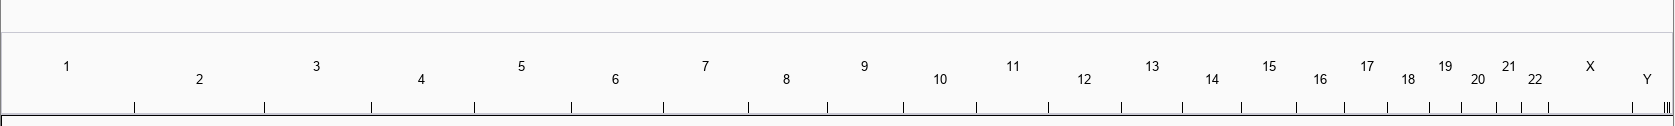
\includegraphics[width=\linewidth]{background/HG.png}
	\caption{The order and the sizes of the chromosomes of the human genome as depicted in the IGV software}
	\label{fig:HG}
\end{figure}

\section{Sequencing}

\subsection{The sequencing technology}

The term \emph{Sequencing} is used for all techniques to read and decipher the DNA code from a given snippet of DNA. During the last years, the techniques that sequence human DNA has changed quite a lot. For about 15 years the \emph{Next Generation Sequencing (NGS)} is the technique most often used. The biggest advantage of NGS, in comparison with other techniques, is the speed of the sequencing since it can sequence billions of short DNA molecules in parallel. In practice, this sequencing is most often done by the instruments of the company Illumina, which dominates the market (around 90\% market share).

\paragraph{How whole-genome NGS works}

\begin{enumerate}
	\item The DNA to sequence is isolated from the cells. Most often this is the whole genome.
	\item  In some cases, The isolated DNA can now be copied enzymatically. This step is repeated until there are enough copies of the same DNA. Usually, this is in the millions or billions of copies.
	
	\begin{figure}[H]
		%src: file:///D:/Erasmus/thesis/interessante%20papers/masterthesis%20BFAST%20op%20FPGA.pdf
		\centering
		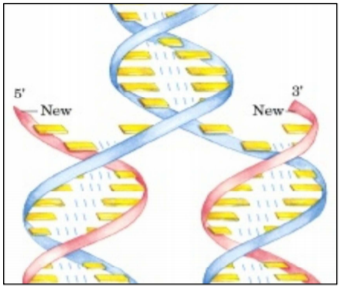
\includegraphics[width=0.3\linewidth]{background/enzymCopying.png}
		\caption{the enzymatic copying of a string of DNA. The original is unzipped, thus allowing new nucleotide bases to attach to the exposed bases.}
		\label{fig:enzymCopying}
	\end{figure}
	
	\item the full DNA sequence is now broken apart into small DNA molecules (100 to 1000 bases long). This is done using enzymes or high-frequency sound waves.
	\item Now the sequencing can start: a \emph{flow cell} is used where these small DNA molecules can bind to a glass surface. 
	\item Different enzymatic and chemical reactions can now be done on this flow cell through an automatic flow of reagents. The following steps are iterated until the full read has been filled in:
	\begin{enumerate}
		\item The entire flowcell is filled with nucleotides, all with different nitrogen bases. Important is that at each of these nucleotides there is a fluorescent group attached. This also makes sure no other nucleotide can bind.
		\item The fluorescent groups have a different color, dependent on the nitrogen base attached ($A$, $G$, $T$ of $C$). At this time a camera picture of the flowcell is taken and stored.
		\item After the flowcell is emptied of the loose nucleotides, another reagent flows in this flowcell. This reagent splits the fluorescent group so that in the next iteration a new nucleotide group can bind with the read.
		
		\begin{figure}[H]
			%src: file:///D:/Erasmus/thesis/interessante%20papers/masterthesis%20BFAST%20op%20FPGA.pdf
			\centering
			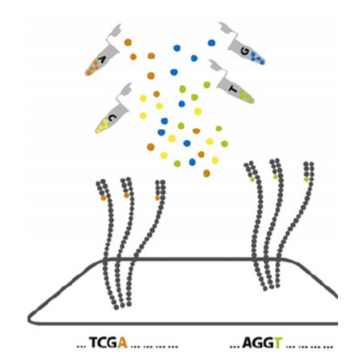
\includegraphics[width=0.5\linewidth]{background/NGS.png}
			\caption{Sequencing technology used by Illumina attaches a nucleotide with a fluorescent tag to the next base in the read, then it captures a picture to determine the base, and removes the fluorescent tag so a new nucleotide group can bind in the next iteration.}
			\label{fig:NGS}
		\end{figure}
	\end{enumerate}
	
	\item After the whole DNA snippets have been filled in, the machine deduces the sequence in the DNA snippet. The pictures that were taken in order during the operation show the colors released in a specific spot, and by extent the attached nitrogen base. By the means of some image processing techniques, it is quite easy to get all the sequences from all the molecules bound on the flowcell. This is called the \emph{Primary processing}.
	
	\begin{figure}[H]
		%src: PPT van Howest
		\centering
		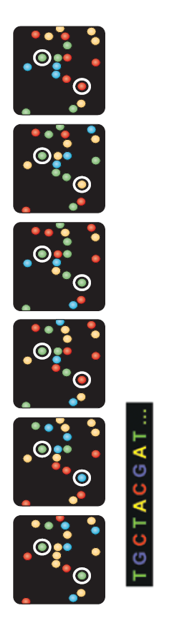
\includegraphics[angle= -90, width=\linewidth]{background/ImProc.png}
		\caption{From left to right is the pictures taken at each iteration in the flowcell. The color at that specific spot marks which nucleotide has been bound. With the use of some image processing techniques the exact sequence in that spot can be identified.}
		\label{fig:ImProc}
	\end{figure}
	
	\item In the \emph{secundary processing}, the sequence is trimmed by quality, etc. The operations that are done on the read in this step are outside the scope of this thesis.
\end{enumerate}

As a result of the NGS, we get a (large) file in the FASTQ format.

\subsection{The FASTQ file format}
\label{expl:FASTQ}

Since the color of each spot observed in the camera pictures in the primary processing can have a light shift, there is a specific "uncertainty" about the correct base is in that spot. This is called the \emph{quality} of the base.

The \emph{FASTQ} file format has become the de-facto standard as output from sequencing instruments. It is a text-based format for storing both the bases in the sequence and their corresponding quality.

A FASTQ file uses four lines per sequenced DNA fragment:

\begin{enumerate}
	\item a '$@$' character followed by a sequence ID, plus an optional description. This description mostly contains the coordinate of the spot on the flowcell.
	\item \label{enumIt:fastqRaw} The sequence of DNA bases identified by the machine. This is either $A$, $G$, $C$, $T$, or $n$ when the base cannot be identified with a specific threshold certainty.
	\item a '$+$' character, optionally followed by the sequence ID (again) and an optional description.
	\item the quality values for each respective base in line \ref{enumIt:fastqRaw}. The length of this line must be the same as the number of bases in line \ref{enumIt:fastqRaw}
\end{enumerate}

The quality score in memory is a value in the range $0x21$ (lowest quality) to $0x7e$ (highest quality). Since this value is represented in ASCII in the file format, this ranges from the '$!$' character to the '$\mathtt{\sim}$' character. Hereunder is a complete list of the possible values of the quality score:

\begin{lcverbatim}
!"#$%&'()*+,-./0123456789:;<=>?@ABCDEFGHIJKLMNOPQRSTUVWXYZ
[\]^_`abcdefghijklmnopqrstuvwxyz{|}~
\end{lcverbatim}


Important to note is that this quality score is logarithmic. Also, the '$@$' and '$+$' character is a possible value for the quality, so this will be something to look out for when implementing the interpreter for this file.\\

	
A FASTQ file containing a single sequence of a DNA fragment of 60 bases might look like this:


\begin{lcverbatim}
@*((((***+))%%%++)(%%%%).1***-+*''))**55CCF>>>>>>CCCCCCC65
\end{lcverbatim}

Keep in mind that a FASTQ file consists of multiple of these sequences, all stacked under each other.
	
	
